\clearpage

\section{M-QAM Receiver}\label{lib:homodyneRx}

\begin{tcolorbox}	
	\begin{tabular}{p{2.75cm} p{0.2cm} p{10.5cm}} 	
		\textbf{Header File}   &:& m\_qam\_receiver.h \\
		\textbf{Source File}   &:& m\_qam\_receiver.cpp \\
        \textbf{Version}       &:& 20190403 (\emph{Bruno Santos})\\
	\end{tabular}
\end{tcolorbox}
\bigbreak
The coherent receiver block receives an optical signal and outputs and electrical binary data. The process of demodulation consists in separating the quadrature and in phase amplitudes and then decode them according to the constellation.


\subsection*{Input parameters}

This block input parameters that can be manipulated by the user in
order to change the configuration of the receiver. Each parameter is changed by
calling a
particular function. 
\begin{itemize}
    \item double rxLocalOscillatorPower\textunderscore dBm( 6 )
    \item double rxTiAmplifierInputNoisePowerSpectralDensity( 1e-16 )
    \item int rxTiAmplifierImpulseResponseTimeLength\textunderscore ( 5 )
    \item double rxTiAmplifierBandwidth( 50.0e9 )
    \item double rxThermalNoisePower( 0 )
    \item pulse\textunderscore shapper\textunderscore filter\textunderscore type rxElectricalFilterImpulseResponseType\newline ( pulse\textunderscore shapper\textunderscore filter\textunderscore type::RaisedCosine )
    
    \item int rxSamplerSamplesToSkip((txPulseShaperLength\textunderscore symbolPeriods-1) x samplesPerSymbol+\newline (rxTiAmplifierImpulseResponseTimeLength\textunderscore symbolPeriods x samplesPerSymbol/2))

\end{itemize}

\subsection*{Signals}
These signals correspond to the Output and since we have to branches, some signals appear twice.
\subsubsection{Inputs}
\subparagraph*{Number:} 0  Optical Signal In
\subparagraph*{Type:} Optical signal
\subparagraph*{Number:} 1 Local Oscillator In
\subparagraph*{Type:} Optical Signal
\bigbreak
\subsubsection{Output}
\subparagraph*{Number:} 5 MQam Receiver Out
\subparagraph*{Type:} Binary Data
\bigbreak
\subsubsection{Internal Signals}
\subparagraph*{Number:} 2 and 4 Optical hybrid Out S + L
\subparagraph*{Type:} Optical Signal
\subparagraph*{Number:} 3 and 5 Optical hybrid Out S - L
\subparagraph*{Type:} Optical Signal
\subparagraph*{Number:} 6 and 7 Balanced Photodetector
\subparagraph*{Type:} Optical Signal
\subparagraph*{Number:} 8 and 9 TI\textunderscore Amplifier
\subparagraph*{Type:} Electrical Signal
\subparagraph*{Number:} 10 and 11 Receiver Filter Out
\subparagraph*{Type:} Electrical Signal
\subparagraph*{Number:} 12 and 13 White Noise Out
\subparagraph*{Type:} Electrical Signal
\subparagraph*{Number:} 14 and 15 Add Out
\subparagraph*{Type:} Electrical Signal
\subparagraph*{Number:} 16 and 17 Sampler Out
\subparagraph*{Type:} Electrical Signal
\bigbreak
\subsection{Methods}
        \begin{itemize}
            \item MQamReceiver(initializer\_list$<$Signal *$>$ \&inputSig, initializer\_list$<$Signal *$>$ \&outputSig)
        \subsubsection{Photodiodes configuration}
            \item void setPhotodiodesResponsivity(t\_real Responsivity)
        \subsubsection{TI\textunderscore Amplifier Configuration}
            \item void setGain(t\_real gain)
            \item void setAmplifierInputNoisePowerSpectralDensity(t\_real NoiseSpectralDensity)
            \item void setTiAmplifierFilterType(Filter fType)
            \item void setTiAmplifierCutoffFrequency(double ctfFreq)
            \item void setTiAmplifierImpulseResponseTimeLength\_symbolPeriods(int irl)
            \item void setElectricalFilterImpulseResponse(vector$<$t\_real$>$ ir)
            \item void setElectricalImpulseResponseFilename(string fName)
            \item void setElectricalSeeBeginningOfImpulseResponse\newline (bool sBeginningOfImpulseResponse)
        \subsubsection{General Noise Configuration}
            \item void setNoiseSamplingPeriod(t\_real SamplingPeriod)
            \item void setNoiseSymbolPeriod(t\_real nSymbolPeriod)
        \subsubsection{Thermal Noise Configuration}
            \item void setThermalNoiseSpectralDensity(t\_real NoiseSpectralDensity)
            \item void setThermalNoisePower(t\_real NoiseSpectralDensity)
            \item void setThermalConstantPower(bool cp)
            \item void setSeeds(array$<$int, 2$>$ noiseSeeds)
            \item void setSeedType(SeedType seedType)
            \item void setThermalConstantPower(bool cp)
        \subsubsection{Pulse Shaper Config}
            \item void setImpulseResponseTimeLength(int impResponseTimeLength)
            \item void setFilterType(pulse\_shapper\_filter\_type fType)
            \item void setRollOffFactor(double rOffFactor)
            \item void usePassiveFilterMode(bool pFilterMode)
            \item void setRrcNormalizeEnergy(bool ne)
            \item void setMFImpulseResponseFilename(string fName)
            \item void setMFSeeBeginningOfImpulseResponse(bool sBeginningOfImpulseResponse)
        \subsubsection{Sampler Configuration}
            \item void setSamplesToSkip(int sToSkip)
        \subsubsection{Decoder Config}
            \item void setIqAmplitudes(vector$<$t\_iqValues$>$
            iqAmplitudesValues)
        \subsubsection{Respective Get Functions}
            \item t\_real getGain(void)
            \item t\_real getAmplifierInputNoisePowerSpectralDensity(void)
            \item double const getElectricalSeeBeginningOfImpulseResponse(void)S
            \item double const getMFSeeBeginningOfImpulseResponse(void)
            \item vector$<$t\_iqValues$>$ const getIqAmplitudes(void)
             \end{itemize}
\clearpage
\subsection*{Example}
\begin{figure}[H]
	\centering
	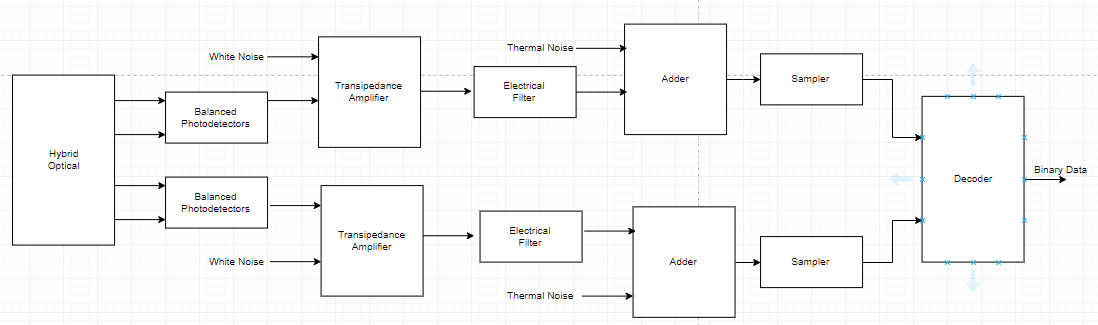
\includegraphics[scale=0.5, height=9cm, width=\textwidth]{../lib/m_qam_receiver/figures/receiver_diagram.png}
	\caption{Simplified model of the MQAM receiver}
	\label{fig:Coherent receiver}
\end{figure}
\begin{figure}[H]
	\centering
	\begin{subfigure}{0.3\textwidth}
		\centering
		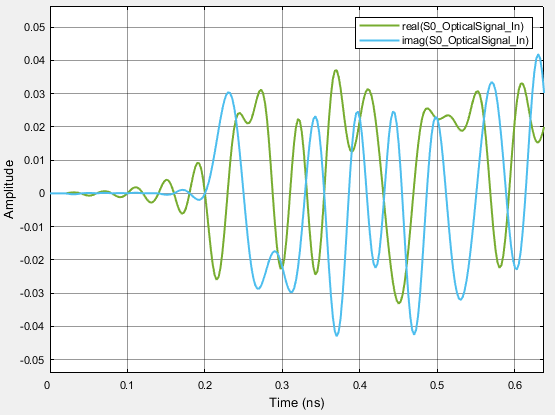
\includegraphics[scale=0.3]{../lib/m_qam_receiver/figures/Optical_in.png}
		\caption{Input of the receiver}
		\label{fig:optical_in}
	\end{subfigure}
	\begin{subfigure}{0.3\textwidth}
		\centering
		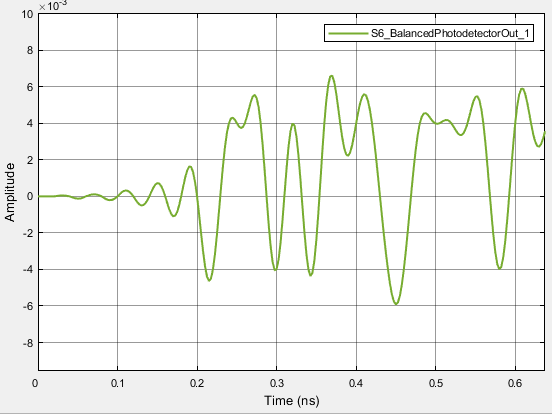
\includegraphics[scale=0.3]{./lib/m_qam_receiver/figures/balance_out.png}
		\caption{Output of the Balanced Photodetectors}
		\label{fig:bal_out}
	\end{subfigure}
	\caption{Internal Signals}
	\label{fig:internal_signals_part1}
\end{figure}


\begin{figure}[H]
	\centering
	\begin{subfigure}{0.3\textwidth}
		\centering
		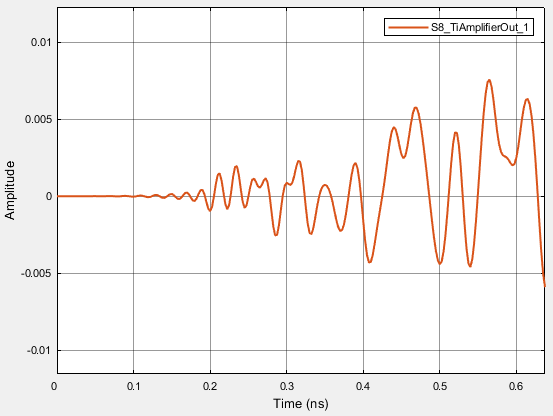
\includegraphics[scale=0.3]{./lib/m_qam_receiver/figures/amp_out.png}
		\caption{Output of Transipedance Amplifier}
		\label{fig:Ti_out}
	\end{subfigure}
	\begin{subfigure}{0.3\textwidth}
		\centering
		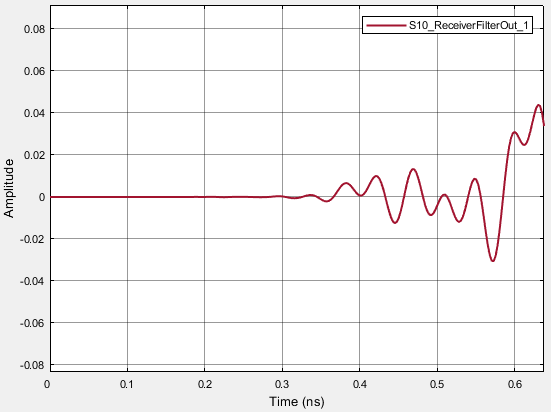
\includegraphics[scale=0.3]{./lib/m_qam_receiver/figures/matched_out.png}
		\caption{Output of the matched filter}
		\label{fig:matched_out}
	\end{subfigure}
\caption{Internal Signals}
\label{fig:internal_signals_part2}
\end{figure}


\begin{figure}[H]
	\centering	
	\begin{subfigure}{0.3\textwidth}
		\centering
		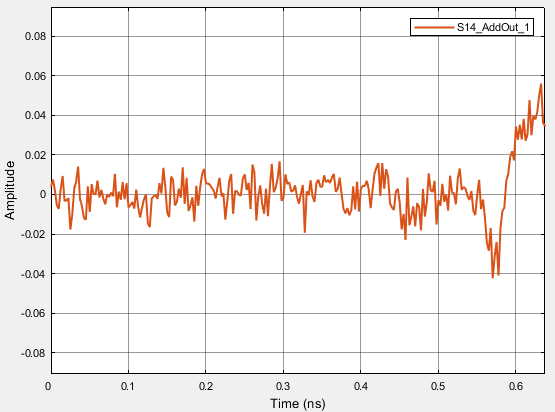
\includegraphics[scale=0.3]{./lib/m_qam_receiver/figures/Add_out.png}
		\caption{Signal with thermal Noise}
		\label{fig:thermal_out}
	\end{subfigure}
	\begin{subfigure}{0.3\textwidth}
		\centering
		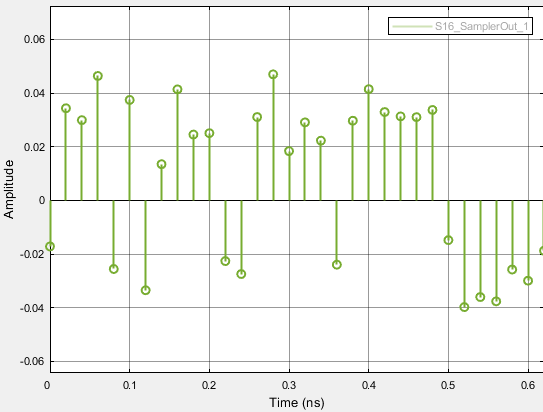
\includegraphics[scale=0.3]{./lib/m_qam_receiver/figures/sampler.png}
		\caption{Digitalization of the signal}
		\label{fig:sampler}
	\end{subfigure}
	\caption{Internal Signals}
	\label{fig:internal_signals_part3}
\end{figure}



\begin{figure}[H]
    \centering
	\begin{subfigure}{0.4\textwidth}
		\centering
    	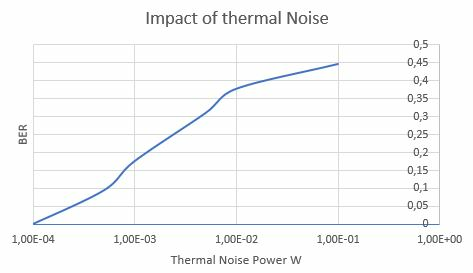
\includegraphics[scale=0.45]{./lib/m_qam_receiver/figures/thermal_noise_ber.png}
    	\caption{Thermal Noise vs BER}
    	\label{fig:thermal}
	\end{subfigure}    
	\begin{subfigure}{0.4\textwidth}
    	\centering
    	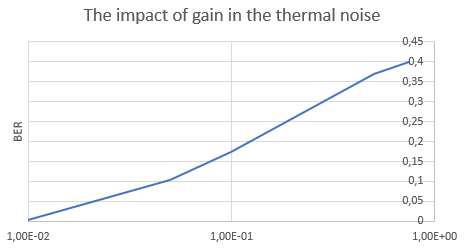
\includegraphics[scale=0.45]{../lib/m_qam_receiver/figures/ber_thermal_gain.png}
    	\caption{Impact of Gain in thermal noise}
    	\label{fig:gainvsthermal}
	\end{subfigure}
\caption{In the \ref{fig:gainvsthermal} with a gain equal to ten, we can see that the impact of the thermal noise is reduced because at the stage where the thermal noise is injected, the signal power is larger than when using unitary gain and we feel less the noise impact}
\label{fig:thermal_compare}
\end{figure}
\pagebreak
\subsection*{Functional description}
This block receives two optical signals, the local Oscillator and the signal coming from the antenna, these two enter on the block \textit{Optical Hybrid} which outputs the sum of the carrier with the signal. Since we must split the signal into quadrature and phase the output is two signals, one of them is real and the other is complex with a phase difference of 90 degrees. In reality it outputs four signals because the next block uses an balanced input.\newline
The block that interprets the optical signal is a \textit{Balanced Photodetector}. This block outputs an electrical signal in baseband because the current produced by the photodetector is proportional to the squared input and since we use a balanced input the result is the product of the local oscillator with the signal. Since its the product of two waves the result is an wave at baseband and other centered at double the frequency. \newline
The next step is converting the current signal into voltage. This is done with an \textit{Transipedance Amplifier} which filters the high band signal and gives power to the signal.\newline
In order to increase the SNR of the signal we use a \textit{Matched Filter} to reduce the noise and then we discretize the signal in order to convert to digital.\newline
The last step is to join the signal in quadrature with the signal in phase and based on the constellation do the respective decision.
\subsubsection{Impact of the thermal noise on the sensitivity}
The temperature at which the receiver is working is bigger than zero K, it means that thermal noise will be generated by the oscillation of the electrons. This has direct impact on the BER as we can see in \ref{fig:thermal}.\newline
We can conclude that the best operating temperatures for an optical receiver are the lowest possible. Later we will see how to reduce the impact of this noise.

\subsubsection{Impact of gain and bandwidth of the \textit{Transipedance Amplifier}}
The Amplifier is the first electrical stage and one of his main characteristics is being low noise. The reason is because the electrical noise generated by the amplifier will also be amplified.\newline
The impact of the bandwidth is simple, if we filter at a frequency where it still has data we will lose some bits and increase the BER.
This stage is very important because if we have high gain we will reduce the impact of the noise injected by the future stages as we can see in \ref{fig:gainvsthermal}
\subsection*{Suggestions for future improvement}

